\documentclass[11pt]{extarticle}
\usepackage[utf8]{inputenc}
\usepackage[T1]{fontenc}
\usepackage[french]{babel}
\usepackage{amsmath,amssymb}
\usepackage{amsfonts}
\usepackage{amssymb}
\usepackage{amsmath}
\usepackage{lmodern}
\usepackage{color}
\usepackage{graphicx}
\usepackage{geometry}
\usepackage{dialogue}
\usepackage{pdfpages}
\usepackage{algpseudocode}
\usepackage{algorithm}
\usepackage{algorithmicx}
\usepackage{listings}
\usepackage{hyperref}

\renewcommand{\algorithmicend}{\textbf{fin}}
\renewcommand{\algorithmicif}{\textbf{Si}}
\renewcommand{\algorithmicthen}{\textbf{Alors}}
\renewcommand{\algorithmicelse}{\textbf{Sinon}}
\renewcommand{\algorithmicfor}{\textbf{Pour}}
\renewcommand{\algorithmicforall}{\textbf{Pour chaque}}
\renewcommand{\algorithmicdo}{\textbf{faire}}
\renewcommand{\algorithmicwhile}{\textbf{Tant que}}
\renewcommand{\algorithmicreturn}{\textbf{Retourner}}


\def\C{\mathbb{C}}
 \parskip 5mm
 \parindent 5mm
 \definecolor{Green}{RGB}{20,127,50}
 \definecolor{Red}{RGB}{150,50,50}
\definecolor{orange}{rgb}{0,0.6,0}
\definecolor{blue}{rgb}{0.1,0.2,0.6}
\definecolor{mauve}{rgb}{0.58,0.5,0.62}
 \geometry{top=40mm, bottom=15mm, left=30mm , right=25mm}
 
 \hypersetup{
    colorlinks=true,       % false: boxed links; true: colored links
    linkcolor=blue,          % color of internal links (change box color with linkbordercolor)
    citecolor=green,        % color of links to bibliography
    filecolor=magenta,      % color of file links
    urlcolor=cyan           % color of external links
}
 
\lstdefinestyle{customc}{
  belowcaptionskip=1\baselineskip,
  breaklines=true,
  frame=L,
  xleftmargin=\parindent,
  language=C++,
  showstringspaces=false,
  tabsize=2,
  basicstyle=\footnotesize,
  keywordstyle=\bfseries\color{Green},
  identifierstyle=\color{blue},
  stringstyle=\color{orange},
  commentstyle=\footnotesize\ttfamily\color{mauve},
}


\newcommand{\intervalle}[2]{\mathopen{[}#1\,;#2\mathclose{]}}
\newcommand{\reelplus}{$\mathopen{[}0\,;+\infty\mathclose{[}$}
\newcommand{\reelmoins}{$\mathopen{]}-\infty\,;0\mathclose{]}$}
\newcommand{\reel}{$\mathopen{]}-\infty\,;+\infty\mathclose{[}$}
\author{\textcolor{Green}{Firegreen}}
\title{\textcolor{Green}{\textbf{Maths}}}

\renewcommand{\familydefault}{\sfdefault}

\geometry{top=20mm, bottom=15mm, left=30mm , right=25mm}
\begin{document}
\begin{minipage}[t]{0.3\paperwidth}
\begin{flushleft}
\raisebox{-0.5\height}{
\includegraphics[width=0.15\paperwidth]{../images/imac}}
\end{flushleft}
\end{minipage}
\begin{minipage}[t]{0.4\paperwidth}
\begin{flushright}
\noindent \Huge{Algorithmique Avancé} \\
\noindent \LARGE{TP 4} \\
\noindent \Large{Tas et Codage de Huffman}
\end{flushright}
\end{minipage}\\
\begin{center}
\rule{\textwidth}{0.2cm}
\end{center}
\section{TP - Exercice 2}

Pour l'exercice 2, vous allez implémenter un codage de Huffman. C'est à dire encoder une chaine de caractères pour obtenir un code composé de '0' et de '1'. Puis faire le processus inverse, c'est à dire à partir de ce code, réobtenir la chaine originale.\\
Pour ce faire vous allez devoir créer un arbre de Huffman et pour en obtenir un efficient, vous allez utiliser un Tas, un Tas-minimum plus précisément, qui va classer les caractères de la chaine selon leur occurrences, en ayant celui avec le moins de fréquence en tête de Tas. Avec ce tas, vous allez prendre 2 par 2 les éléments les plus petits pour en faire des sous-arbre avec un nouveau noeud parent qui va être réinséré dans le tas. On répète le processus jusqu'à ne plus avoir de couple de caractères dans le tas.

\begin{center}
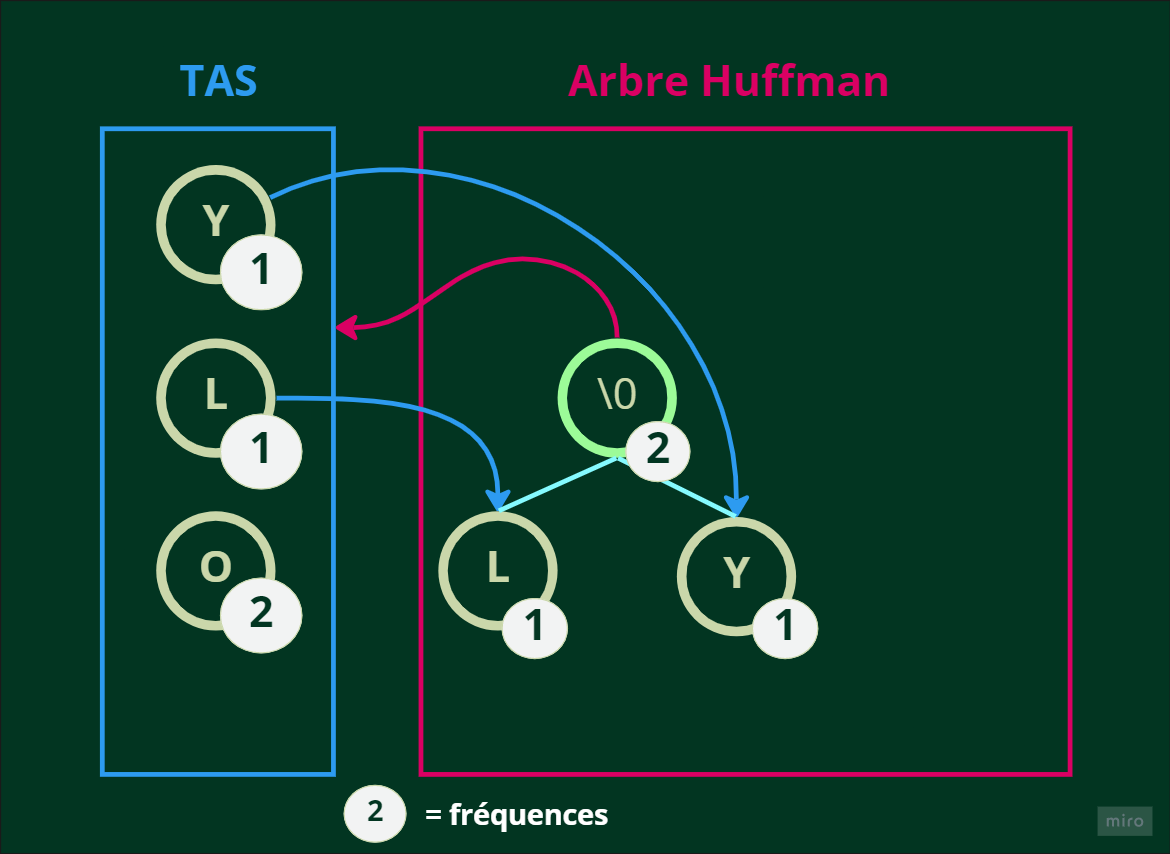
\includegraphics[width=0.48\textwidth]{images/huffman_heap.png}
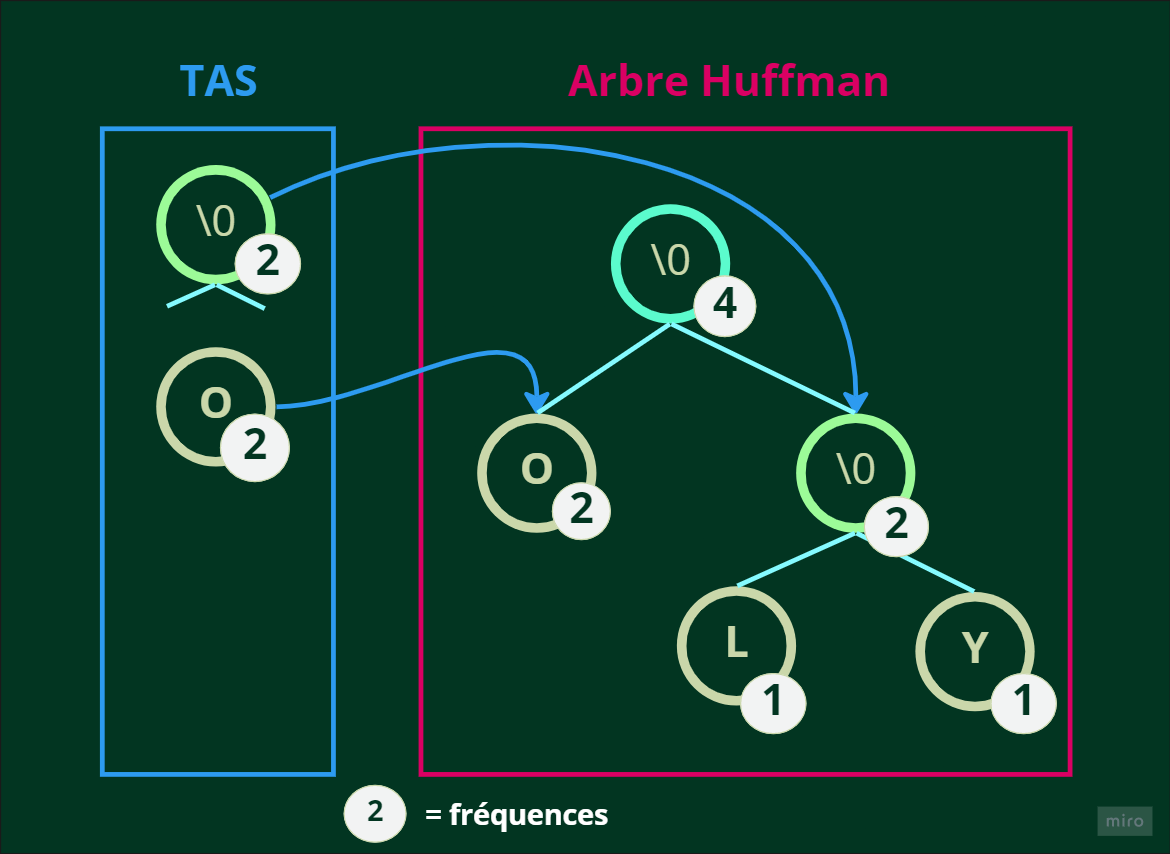
\includegraphics[width=0.48\textwidth]{images/huffman_heap2.png}
\end{center}
\newpage
Pour y arriver, implémentez un certains nombres de fonctions décrites plus bas.\\
Pour faire fonctionner ces fonctions vous aurez besoin d'une structure \textit{HuffmanHeap} et \textit{HuffmanNode}.\\
\textit{HuffmanNode} est un noeud d'arbre possédant les attributs $character$, $value$ et $code$ qui sont respectivement le caractère représentant le noeud, la fréquence d'apparition de ce caractères et le code produit par le dictionnaire. \\
\textit{HuffmanHeap} est un tas de \textit{HuffmanNode} utilisant la fréquence d'un caractères pour les ordonner.

\begin{itemize}

\item[ - \textbf{processCharFrequences}(string $data$, Array $frequences$)]: Rempli chaque case $i$ de $frequences$ avec le nombre d'apparition du caractère correspondant au code ASCII $i$ dans la chaine de caractère $data$.
\item[ - \textbf{insertHeapNode}(HuffmanHeap $heap$, int $heapSize$, HuffmanNode* $node$)]: Insère un nouveau HuffmanNode dans le tas-minimum en utilisant la $frequence$ comme priorité.
\item[ - \textbf{buildHuffmanHeap}(Array $frequences$, HuffmanHeap $heap$)]: Construit un tas $heap$ minimum à partir des fréquences d'apparition non nulles de caractères. Un tas minimum est un tas qui donne la priorité aux valeurs les plus basses $\rightarrow$ chaque nœud est plus petit que ses fils.
\item[ - \textbf{heapify}(HuffmanHeap $heap$,  int $heapSize$, int $nodeIndex$)]: répare un tas en partant de l'index donné.
\item[ - \textbf{extractMinNode}(HuffmanHeap $heap$,  int $heapSize$)]: récupère la plus petite valeur (la tête normalement), l'enlève du tas et répare le tas après l'extraction.

\item[ - \textbf{makeHuffmanSubTree}(HuffmanNode* $right$, HuffmanNode* $left$)]: Construit un sous arbre de huffman à partir de deux nodes.
\item[ - \textbf{buildHuffmanTree}(HuffmanHeap $heap$, HuffmanNode* $tree$)]: Construit un dictionnaire de Huffman.
\item[ - \textbf{processCodes}(HuffmanNode $tree$)]: Détermine et définit les codes de toutes les feuilles de $tree$

\item[ - \textbf{huffmanEncode}(string $toEncode$, HuffmanNode* $huffmanTree$)]: Retourne la chaine de caractère encodé à partir des codes se trouvant dans $characters$. $characters$ est un tableau de HuffmanNode*, chaque indice $i$ correspond au code ASCII $i$. 
\item[ - \textbf{huffmanDecode}(HuffmanNode* $huffmanTreeRoot$, string $toDecode$)]: Retourne la chaine de caractère décodé partir du dictionnaire $dict$
\end{itemize}\vspace{1cm}


Si vous êtes chaud patate, renvoyez la chaine de caractère encodé sous forme binaire plutôt que sous forme de caractère. Le but étant de compresser vous devez utilisez un octet plus stocker plusieurs caractères. N'hésitez à appeler votre chargé de TD préféré pour avoir plus d'informations (parce que la flemme d'expliquer par écrit).
Vous pouvez utiliser le langage que vous souhaitez.
\subsection{C++}
Le dossier \textit{Algorithme\_TP4/TP} contient un dossier \textit{C++}. Vous trouverez dans ce dossier des fichiers \textit{exo<i>.pro} à ouvrir avec \textit{QtCreator}, chacun de ces fichiers projets sont associés à un fichier \textit{exo<i>.cpp} à compléter pour implémenter les différentes fonctions ci-dessus. \\
L'exercice \textit{exo1.cpp} implémente une structure \textit{Heap} possédant les différentes méthodes d'un tas à implémenter. \\
Cette structure est une spécialisation de \textit{Array}, il possède donc les mêmes fonctions d'accès que lui.
\begin{lstlisting}[style=customc, escapechar=@]
class Heap : public Array {

	void print(); // declaration de la methode print de Heap

}

void Heap::print() // corps de la methode print de Heap
{
	for (i=0; i < this->size(); ++i)
		printf("%d ", this->get(i));
}

void Heap::clear() // corps de la methode clear de Heap
{
	for (i=0; i < this->size(); ++i)
		this->set(i, 0);
}
\end{lstlisting}
\textit{HuffmanHeap} est un tas qui plutôt de stocker des entier, stocker des HuffmanNode. \\
\textit{HuffmanNode} est un noeud, comme \textit{BinaryTree} dans le TP3, il possède un enfant gauche $left$ et droit $right$ du même type que lui, ces deux enfants peuvent donc utiliser les mêmes méthodes que \textit{HuffmanNode}. \\
\begin{lstlisting}[style=customc, escapechar=@]
struct HuffmanNode {
	
	HuffmanNode* left;
	HuffmanNode* right;	
	int value;
	char character;
	string code;
	
	void print()
	{
		if (this->left != nullptr)
			printf("left: %d with code: %s\n", this->left->value, this->left->code);
		if (this->right != nullptr)
			printf("right: %d with code: %s\n", this->right->value, this->right->code);
		printf("this: %d\n", this->value);
	}

}
\end{lstlisting}
\paragraph{Notes:} 
\begin{itemize}
\item Dans une fonction $C_{++}$, si le type d'un paramètre est accompagné d'un '\&' alors il s'agit d'un paramètre entré/sortie. La modification du paramètre se répercute en dehors de la fonction.
\item La fonction $huffmanDict$ a pour paramètre un $HuffmanNode*\&$, il s'agit d'un pointer dont vous pouvez modifier l'adresse vers laquelle il pointe.
\item Lorsque vous faites appel à $this$ dans une méthode d'une structure (ou d'une classe), vous pouvez accéder aux attributs de la structure en question, comme dans l'exemple ci-dessus.
\end{itemize}

\end{document}